\documentclass{standalone}

\usepackage{tikz}
\usetikzlibrary{positioning, arrows.meta}

\begin{document}
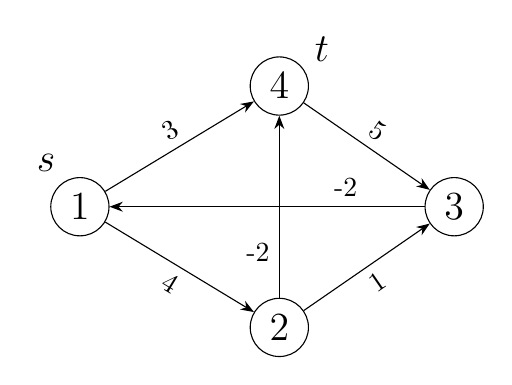
\begin{tikzpicture}[v/.style = {circle, draw, font = \Large},
	e/.style = {>=Stealth, ->}]
  \node (1) [v, label = 120:{\Large $s$}] {1};
  \node (2) [v, below right = 1.0cm and 2.0cm of 1] {2};
  \node (3) [v, right = 4.0cm of 1] {3};
  \node (4) [v, above right = 1.0cm and 2.0cm of 1, label = 30:{\Large $t$}] {4};

  \draw[e] (1) to node[below, sloped] {4} (2);
  \draw[e] (1) to node[above, sloped] {3} (4);
  \draw[e] (2) to node[below, sloped] {1} (3);
  \draw[e] (2) to node[left, near start] {-2} (4);
  \draw[e] (3) to node[above, near start] {-2} (1);
  \draw[e] (4) to node[above, sloped] {5} (3);
\end{tikzpicture}
\end{document}